\section{Students}
\Warning{}
\\After the login you will notice that a black bar has appeared near the top of the screen.
The black bar contains on its left the voices \textbf{Yours exams list} and \textbf{School records}.

\subsection{Visualize the exams list}
To see your exams list click on the voice \textbf{Yours exams list}, you will be redirected to a page (similar to the one in Figure~\ref{fig:studentExams}) that shows the exam to which you can register and to which you are already registered. 
\begin{figure}[!h]
\centering
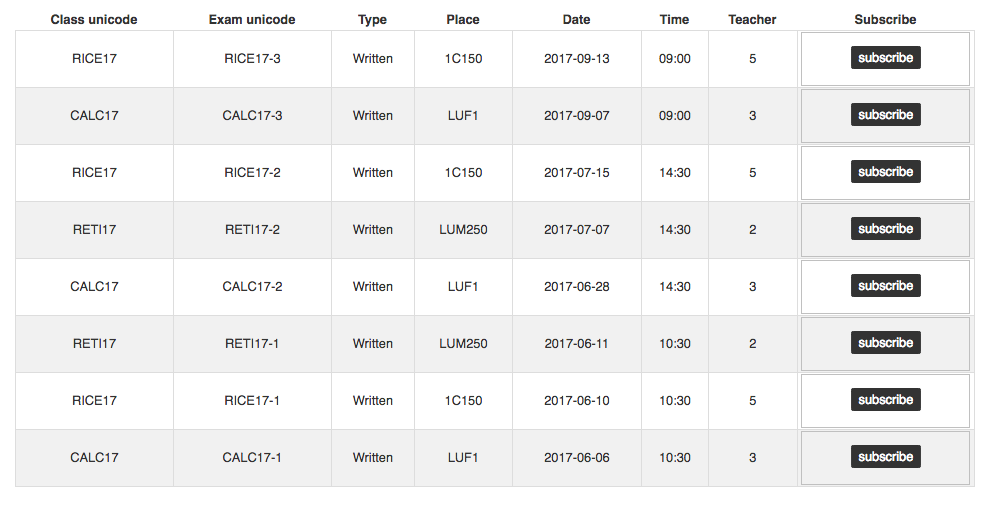
\includegraphics[width=0.65\textwidth]{img/studentExams.png}
\caption{List of exams to which the student can register and to which is already registered.}
\label{fig:studentExams}
\end{figure}

\subsection{Visualize the school records}
If you want to visualize the exams that you have already passed click on the voice \textbf{School records}, you will be redirected to a page (similar to the one in Figure~\ref{fig:studentRecords}) that shows all the exams that you can take. If the cells of the column named \emph{status} are green, then you have passed those exam, otherwise you have not, in this way, you have a direct feedback regarding your university career.

\begin{figure}[!h]
\centering
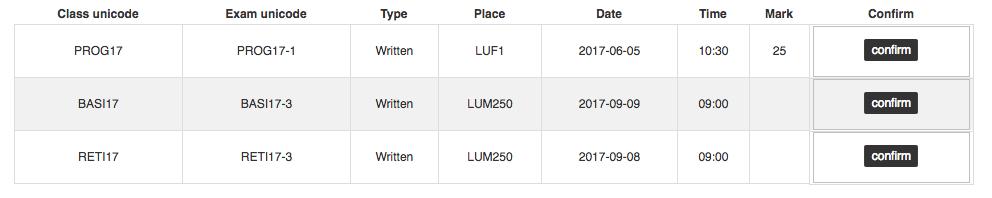
\includegraphics[width=0.65\textwidth]{img/studentRecords.png}
\caption{List of the exams that the student has passed (status cell in green) and hasn't passed (status cell in yellow) }
\label{fig:studentRecords}
\end{figure}